% =====================================================================
% arXiv submission - Primary category: cs.SE
% Full English manuscript (extends the Zenodo preprint, DOI 10.5281/zenodo.22551156).
% Compile with pdfLaTeX. Figures in ./figuras (5 PNG files).
% Uses inline thebibliography -> no BibTeX/Bib file needed server-side.
% =====================================================================
\documentclass[11pt]{article}

\usepackage[utf8]{inputenc}
\usepackage[T1]{fontenc}
\usepackage{amsmath,amssymb}
\usepackage{newtxtext,newtxmath}
\usepackage[margin=1in]{geometry}
\usepackage{graphicx}
\usepackage{booktabs}
\usepackage{microtype}
\usepackage[colorlinks=true,linkcolor=blue,citecolor=blue,urlcolor=blue]{hyperref}
\graphicspath{{figuras/}}

\hypersetup{
  pdftitle={Empirical Evaluation of Quality and Defects in Software Generated by AI Agents: A Comparative Study under Controlled Requirements},
  pdfauthor={Bruno Bertin Marquez}
}

\newcommand{\paperfirst}{sec}

\begin{document}

\begin{titlepage}
  \begin{center}
    {\LARGE\bfseries Empirical Evaluation of Quality and Defects in Software Generated by AI Agents: A Comparative Study under Controlled Requirements\par}
    \vspace{1.2em}
    {\large Bruno Bertin Marquez\thanks{ORCID: \href{https://orcid.org/0009-0005-3546-8302}{0009-0005-3546-8302}. Independent researcher --- Graduate in Software Quality Management (lato sensu); M.S. student in Requirements Engineering (in progress).}\\[0.3em]
    Independent Researcher\par}
  \end{center}
\end{titlepage}

\begin{abstract}
Source code generated by large language models (LLMs) has become routine in the software engineering (SE) lifecycle. The literature has shown, in isolated fragments, that this code exhibits characteristic defect patterns, frequent security vulnerabilities, accumulation of technical debt, tests with limited effectiveness, and imperfect reproducibility. However, no reviewed study combines, in the same controlled experimental chain, the generation of \emph{complete systems} by different \emph{AI agents} from the \emph{same requirement}, under \emph{multiple executions}, evaluated by an \emph{independent oracle} with simultaneous coverage of functionality, defects, security, maintainability, and reproducibility. This paper presents a controlled, prospective, and reproducible experiment that fills that gap: four agents (distinct models executed in the same agent framework \texttt{opencode}, 2$\times$~Nemotron, Ling, and Mimo) each produced three independent executions of a complete system (task-management REST API in Python/FastAPI/PostgreSQL), totaling 12 deliveries evaluated by an independent 81-test oracle suite, plus non-functional verifications (security, maintainability, reproducibility, performance) and a defect matrix classified according to the Tambon et al.\ taxonomy with severities and inter-rater agreement. Results: only 3 of the 12 deliveries were bootable; the 12 Tambon defects were 100\% Blocker or Critical; the tests generated by the agents themselves detected none of the defects (0/12), while the oracle detected 4/4 of the reachable ones (RQ6/H3); recurring patterns (missing dependency; \textit{passlib}+\textit{bcrypt} incompatibility; migration misconfiguration; ``ghost'' version) concentrate most defects and repeat across ``free'' models, suggesting a common ``quality trough'' at collection time. The study descriptively supports that approval by the agents' own tests is no substitute for independent validation, and that a single index would collapse quality dimensions (functional vs.\ global). Statistical power is limited ($n=12$; expected cells $<$5), so H1--H3 are presented as trends, not conclusions; a complementary laboratory study (non-evidential) reinforces the separation between \emph{detecting} and \emph{testing}.
\end{abstract}

\noindent\textbf{Keywords:} AI-generated software; coding agents; software quality; defects; independent oracle; software testing; software engineering; controlled experiment.

\tableofcontents

\section{Introduction}\label{sec:intro}

Large language models (LLMs) now permeate virtually the entire software engineering lifecycle, with concentration in code generation, test generation, and program repair~\cite{A01}. Consolidated systematic reviews point to recurring limitations---hallucinations, security vulnerabilities, poor generalization, and interpretability problems~\cite{A02}. This field, however, presents a conflict of results that remains open: there is evidence \emph{favorable} to AI (GitHub's controlled experiment with Copilot~\cite{D03}; lower estimated repair effort in some scenarios~\cite{D02}) and evidence \emph{unfavorable} (distinct defect profiles at scale~\cite{B03}; frequent vulnerabilities~\cite{E01,E02,E03}). The absence of consensus is precisely what justifies a controlled empirical investigation.

On the \textbf{defects} front, empirical studies have shown that LLM-generated code has characteristic and recurring patterns. Tambon et al.~\cite{B01} analyzed 333 bugs of CodeGen, PanGu-Coder, and Codex and proposed a taxonomy of \textbf{ten defect patterns} (\emph{misinterpretation, syntax error, silly mistake, prompt-biased code, missing corner case, wrong input type, hallucinated object, wrong attribute, incomplete generation, non-prompted consideration}), validated by 34 researchers and practitioners. At a much larger scale, Cotroneo, Improta, and Liguori~\cite{B03} compared more than 500 thousand human and AI code samples and concluded that \textbf{AI and humans have different defect profiles}---AI tends toward more unused constructs, hardcoded debugging, and high-risk security vulnerabilities. Furthermore, LLM results are \textbf{non-deterministic}: the same input can produce different outputs, affecting correctness and scientific reproducibility~\cite{B04}.

On the \textbf{testing} front, the literature is equally cautious. LLM-generated tests may contain \emph{test smells} even when valid~\cite{C03}; their defect-detection ability is limited (29--60\% of detectable defects in Defects4J projects~\cite{C04}); and traditional coverage and \emph{mutation score} metrics lose reliability when the code under test contains a bug~\cite{C05}. Distinct models tend to omit tests of special values (\emph{None, inf, NaN})~\cite{C06}---a direct echo of the \emph{missing corner case} category in the Tambon taxonomy~\cite{B01}.

On the \textbf{non-functional quality} front, the literature privileges functional correctness and underrates security, performance, and especially maintainability and technical debt~\cite{D04}; AI code accumulates \emph{code smells} that persist over time~\cite{D05}. On the \textbf{security} front, breaches are frequent: from 29.5\% (Python) to 24.2\% (JavaScript) of vulnerable snippets~\cite{E01}; all analyzed LLMs generating vulnerabilities, many of high or critical severity~\cite{E02}; and security prompting strategies that shift the distribution but do not significantly reduce vulnerability density~\cite{E03}.

On the \textbf{programming agents} front, the field has moved from ``LLM answers a question'' to ``agent executes real development tasks''. These agents perform refactorings~\cite{F01}, produce projects with limited reproducibility---only 68.3\% run immediately in a clean environment, with a mean $13.5\times$ expansion between declared and required dependencies~\cite{F02}---and fail unevenly across agents: the commit reversion rate ranges from 0.7\% (Codex) to 7.6\% (Copilot)~\cite{F05}.

\textbf{The gap.} The fragments above were demonstrated in isolation. Yet no reviewed study (0/25 in our review---see Sec.~\ref{sec:related}) unites these dimensions in a \textbf{single controlled, reproducible experiment} with the same specification $\rightarrow$ different agents $\rightarrow$ complete systems $\rightarrow$ $\geq$3 executions $\rightarrow$ independent oracle $\rightarrow$ defects + security + maintainability + reproducibility $\rightarrow$ statistical analysis (gaps G1--G5). Retrospective studies observe real data (e.g.,~\cite{D05,F04,F05}) but do not run an experiment with identical requirements and opportunities across groups; most studies work with \emph{snippets}, functions, or \emph{patches}, not \textbf{complete systems}; and few separate who \textbf{generates} from who \textbf{evaluates} with an oracle independent of the generating AI.

\textbf{Research problem.} Stated with due neutrality:

\begin{quote}
Although the literature shows that AI-generated code has characteristic defects, frequent vulnerabilities, and tests with low detection ability, \textbf{there is no controlled empirical evidence on how different AI agents compare when producing complete systems from the same requirements}, evaluated by an \textbf{independent oracle}, under \textbf{multiple executions}, covering simultaneously \textbf{functional quality, defects, security, maintainability, and reproducibility}.
\end{quote}

\textbf{General objective.} Empirically evaluate the quality and defects present in software systems produced by different AI agents/models under controlled experimental conditions (same requirement, same prompt, multiple executions, independent oracle). Specific objectives: compare agents in generation from the same requirement; identify and classify defects (Tambon taxonomy + severity); evaluate testing effectiveness without relying solely on coverage/mutation; evaluate structural quality (ISO/IEC 25010), security (CWE/OWASP), and reproducibility; investigate the AI's ability to detect its own defects; and statistically compare results across agents.

\textbf{Contributions.} (i)~First controlled, prospective, reproducible experiment---as far as the review reaches---that combines, in the same chain, complete systems + defects + security + maintainability + reproducibility + multiple executions + independent oracle; (ii)~empirical evidence of \textbf{recurring defect patterns transferable across ``free'' models} of the same agent pipeline, including a common ``quality trough''; (iii)~evidence on the \textbf{testability} of generated systems (RQ6/H3): the agents' own tests detected no defect, while the independent oracle detected all reachable ones.

\section{Related Work}\label{sec:related}

We condense the review into thematic groups; full entries with DOIs are in Sec.~\ref{sec:refs}. Review-method details and the 25 sources are documented in the research artifacts (matrix and bibliographic review).

\textbf{A---LLMs in Software Engineering.} Hou et al.~\cite{A01} conducted the largest SLR of the field (395 articles, 85 SE tasks across six activities), mapping models, datasets, prompting strategies, and evaluation challenges. Umama et al.~\cite{A02} reviewed 58 studies (PRISMA) and listed recurring limitations (hallucination, security, generalization, interpretability). These SLRs supply the RQ vocabulary of this study but do not conduct a controlled experiment comparing agents in complete-system generation.

\textbf{B---Defects in LLM-generated code.} Tambon et al.~\cite{B01} consolidated the ten-pattern taxonomy we adopt to classify defects. Dou et al.~\cite{B02} showed that bugs vary between benchmarks and real situations, and that self-correction improves passing (+29.2\%), signaling a variable (review by the AI itself) that we keep \emph{out} of the first version of our design to preserve control. Cotroneo et al.~\cite{B03} established that AI and humans have \textbf{different defect profiles}, motivating us to compare distributions (profile), not only totals. Ouyang et al.~\cite{B04} demonstrated \textbf{non-determinism}, justifying our $\geq$3 executions per model.

\textbf{C---LLM-based testing.} Wang et al.~\cite{C01} mapped LLM applications in testing. Beer et al.~\cite{C02} evaluated code and tests generated by ChatGPT/Copilot (small algorithms), finding differences per model/language---we advance to \textbf{complete system} with independent oracle. Alves et al.~\cite{C03} showed \emph{test smells} even in valid tests; Yang et al.~\cite{C04} quantified limited detection (29--60\%); Zhao et al.~\cite{C05} contested the reliability of coverage/mutation in the presence of bugs; Walczak et al.~\cite{C06} showed the omission of special values. Together, they support the testability (C) dimension and the decision \textbf{not} to trust isolated coverage or the AI's own tests.

\textbf{D---Software quality.} Tosi~\cite{D01} evaluated AI engines and concluded on the need for expert supervision (methodological base). Molison et al.~\cite{D02} show that AI can be better/equal/worse depending on context (fostering our neutrality). GitHub's controlled experiment~\cite{D03} favored AI on web endpoints, preventing a hasty conclusion against AI. Sun et al.~\cite{D04} advocated adopting ISO/IEC 25010 and showed the underrating of non-functional aspects---we adopt ISO/IEC 25010 as reference. Liu et al.~\cite{D05} quantified technical debt (89.1\% \emph{code smells}) in AI commits.

\textbf{E---Security.} Fu et al.~\cite{E01} and Morkonda et al.~\cite{E02} quantified vulnerabilities; Kharma et al.~\cite{E03} showed that security prompting does not significantly reduce density. Although our oracle includes a security layer, the prompt given to the agents does \emph{not} instruct on security (to avoid inducing groups unequally).

\textbf{F---Programming agents.} Horikawa et al.~\cite{F01} distinguished agent model (relevant to our framing: we compare models within the same agent framework). Vangala et al.~\cite{F02} showed limited reproducibility (68.3\% run) and a $13.5\times$ dependency expansion---our study measures reproducibility as a dimension (RQ7). Belozerov et al.~\cite{F03} separated requirement error from AI-introduced error. Ehsani et al.~\cite{F04} and Oukhay et al.~\cite{F05} showed that real agents behave unevenly (reversions 0.7\%--7.6\%), reinforcing the relevance of comparing distinct treatments.

\textbf{Gaps (G1--G5) and position of this study.} The full review supporting this work (25 articles: 16 with journal/conference DOI, 8 preprints, 1 institutional report) reveals that 8\% of studies generate a \textbf{complete system}, 12\% use an \textbf{independent oracle}, and 0\% combine complete system + defects + security, nor run the full design (spec$\rightarrow$agents$\rightarrow$$\geq$3 executions$\rightarrow$oracle$\rightarrow$defects+NFR$\rightarrow$statistics). We position this experiment exactly in that gap (G1--G5; see research artifacts for the quantitative matrix analysis).

\section{Methodology}\label{sec:method}

\subsection{Methodological position, neutrality, and pre-registration}

Controlled, prospective, and reproducible experiment (unlike retrospective studies such as~\cite{D05,F04,F05}). The hypotheses, RQs, analysis plan, exclusion criteria, and the neutrality principle were fixed \textbf{before} data collection (problem-and-hypotheses and methodology documents committed beforehand in the research repository) and later consolidated as a pre-registration \textbf{formalized retrospectively}, with temporal anchors verifiable in the git history (the results section was added in a separate commit). \textbf{Neutrality (C1):} the experiment does not start from ``AI is bad''; if the data shows AI equal or better on some dimension, that is a result, not a limitation.

\subsection{Experimental design}

\begin{itemize}
  \item \textbf{Type:} between-groups comparison (one group per agent), with repetitions within the group.
  \item \textbf{Experimental unit:} a \textbf{complete system} (REST API) generated by an agent from the specification.
  \item \textbf{Treatment (independent variable):} model identity within the agent.
  \item \textbf{Replications:} \textbf{3 independent executions per agent} (addresses non-determinism~\cite{B04} and RQ8).
  \item \textbf{Blinding:} oracle written by independent QA and kept in a private repository, outside agents' reach (avoids \emph{data leakage}; cf.~\cite{C06}).
\end{itemize}

\textbf{Agents (treatments).} To reduce tool confounding, all treatments use the \textbf{same agent framework} (\texttt{opencode}---same read/edit/test loop), varying only the \textbf{model}. Four ``free'' models from distinct families (2$\times$~Nemotron, Ling, Mimo):

\begin{table}[htbp]
  \centering
  \caption{Agents (treatments).}
  \label{tab:agents}
  \begin{tabular}{ll}
    \toprule
    Model & \texttt{opencode} ID \\
    \midrule
    Nemotron 3 Ultra (NVIDIA) & \texttt{opencode/nemotron-3-ultra-free} \\
    Nemotron 3.5 Lightning (NVIDIA) & \texttt{opencode/nemotron-3.5-lightning-free} \\
    Ling 3.0 Flash & \texttt{opencode/ling-3.0-flash-fin-free} \\
    Mimo v2.5 & \texttt{opencode/mimo-v2.5-free} \\
    \bottomrule
  \end{tabular}
\end{table}

The exact version of each model is recorded per execution in the manifest (agents have versions;~\cite{F05} showed differences). Declared limitation: agent-tool comparison is lost (mitigated by the identical \texttt{opencode} loop).

\subsection{Controlled specification (the ``same requirement'')}

Target system: \textbf{Task-Management REST API} (moderate and realistic scope), in Python + FastAPI + PostgreSQL. Functional requirements (FR1--FR8): registration/login with hash and JWT; task CRUD; permission rules (owner/admin); filters and pagination; input validation; standardized error handling; PostgreSQL persistence with migrations; automated tests in the delivery. Non-functional requirements (NFRs) anchored in ISO/IEC 25010~\cite{D04} and CWE/OWASP~\cite{E01,E02,E03}: security, maintainability, reproducibility, basic performance. The specification is the \emph{only} document given to the agents, in identical format. NFRs are informed only with behavioral acceptance criteria, \emph{without} ``solution'', to avoid inducing groups unequally.

\subsection{Independent oracle}

Suite \textbf{independent of the generating AI}, private and immutable during collection, validated against a golden (non-AI) reference system. Layers:

\begin{table}[htbp]
  \centering
  \caption{Independent oracle layers.}
  \label{tab:oracle}
  \begin{tabular}{lll}
    \toprule
    Layer & Content & Tool \\
    \midrule
    Functional & Unit, integration, API covering FR1--FR8 and acceptance cases & pytest, pytest-cov, httpx \\
    Negative & \emph{Invalid input}, extremes (\emph{None/inf/NaN}), permissions, authentication & parametrized pytest \\
    Security & Authentication/authorization, injection, dependencies & bandit, pip-audit \\
    Structural & Complexity, duplication, \emph{code smells}, maintainability & Ruff + radon \\
    Testability & Agent's own tests run against the oracle; real detection rate & pytest \\
    \bottomrule
  \end{tabular}
\end{table}

Rules: not reviewed by the agent; not exposed in the prompt; covers all FR/NFR; \textbf{coverage is reported but not treated as quality evidence}~\cite{C05}; only real defect detection is credited. The suite has \textbf{81 tests} and is strictly \emph{black-box} with respect to the backend.

\textbf{Validation environment (D9).} The execution machine is a VM \emph{without nested virtualization}; therefore validation was \emph{native} (native PostgreSQL + venv + \texttt{alembic upgrade head} + uvicorn + \texttt{/health} gating). Docker artifacts required in the delivery remain mandatory and are validated structurally; they will be executed in containers on the production machine. This condition is reported as a limitation (Sec.~\ref{sec:limitations}).

\subsection{Defect matrix and classification}

Each defect is recorded with: ID; agent + execution; location; \textbf{category} (Tambon taxonomy, 10 patterns~\cite{B01}); \textbf{severity} (Blocker/Critical/Major/Minor, harmonized with CWE for security); \textbf{detection} (by oracle? by agent's tests?); evidence (reproducing test). \textbf{Independent double classification} by two raters, with Cohen's $\kappa$ and divergence resolution in meeting. Density = defects per KLOC of the delivered project (LOC snapshotted, without \emph{venv}/cache).

\subsection{Metrics and statistical analysis}

RQ$\rightarrow$metric$\rightarrow$instrument mapping and pre-defined tests:

\begin{table}[htbp]
  \centering
  \caption{RQs, hypotheses, metrics, and tests.}
  \label{tab:rq}
  \begin{tabular}{lll}
    \toprule
    RQ/H & Metric & Test/Instrument \\
    \midrule
    RQ1 functional & Oracle pass rate per execution & pytest \\
    RQ2/H1 density & Defects/KLOC per agent & descriptive + Poisson CI (small $n$) \\
    RQ3/H2 categories & Category distribution per agent & $\chi^2$ + Cram\'er's $V$; pointwise Fisher exact \\
    RQ4 severity & Severity distribution & descriptive; \% Blocker/Critical \\
    RQ5/H4 global & Functional vs.\ NFR (separate dimensions) & per-dimension comparison; no single index \\
    RQ6/H3 testability & Defects detected by agent's tests vs.\ oracle & $2\times2$ matrix; Fisher exact \\
    RQ7 reproducibility & Runs in clean environment; instructions; dependencies & executability check \\
    RQ8 variability & Variance across the $\geq$3 executions & descriptive (CV) \\
    \bottomrule
  \end{tabular}
\end{table}

Significance level $\alpha=0.05$ with multiple-comparison correction. Honest rule: $\chi^2$ is only conclusive with expected cells $\geq$5; with expected cells $<$5 we use Fisher exact and \textbf{report as informative, not conclusive}. Negative results are reported as results (neutrality).

\subsection{Collection procedure}

(1)~freeze specification v1.0 and oracle (private, immutable); (2)~for each agent, new session with the same prompt (``implement the specification; deliver an executable system with tests''); (3)~$\geq$3 independent sessions per agent; (4)~capture agent/model version, prompt, log, repository, and delivered tests; (5)~evaluate each delivery only with the oracle and the matrix (raters blind to agent when possible); (6)~record evidence. Exclusion criteria: \textbf{pilot} executions; \textbf{infrastructure} findings (e.g., session rejected by permission; VM disk full); \textbf{NFR/non-bug} findings (classified separately). Phases: specification $\rightarrow$ oracle+golden $\rightarrow$ pilot (calibration) $\rightarrow$ full run ($4\times3$) $\rightarrow$ classification/analysis $\rightarrow$ consolidation.

\subsection{Threats to validity and mitigation}\label{sec:threats}

Oracle \emph{data leakage} (private/immutable oracle); non-determinism ($\geq$3 executions); agent confounding (same requirement/prompt/environment); model change during the study (freeze versions); low statistical power (report effect size, $n=3$/agent); rater bias (double classification, $\kappa$, blind raters, pre-registration); oracle embedding solutions (written from the specification and validated against golden); publication bias (pre-registration); too-easy/too-hard scope (moderate specification + pilot).

\section{Results}\label{sec:results}

We ran \textbf{12 complete deliveries (4 agents $\times$ 3 executions)}; calibration pilots were \textbf{excluded} from analysis. Tables and figures accompany this text (Figures~\ref{fig:density}--\ref{fig:severity}, generated by a reproducible script from the aggregates).

\subsection{Delivery characterization and functional quality (RQ1)}

\begin{table}[htbp]
  \centering
  \caption{Delivery characterization (oracle execution).}
  \label{tab:delivery}
  \begin{tabular}{lccccc}
    \toprule
    Execution & Tests & Failures & Errors & Passed & Boot \\
    \midrule
    lightning/e1--e2 & 0 & 0 & 0 & 0 & no \\
    \textbf{lightning/e3} & \textbf{81} & \textbf{32} & \textbf{48} & \textbf{1} & \textbf{yes} \\
    ling/e1--e3 & 0 & 0 & 0 & 0 & no \\
    \textbf{mimo/e2} & \textbf{81} & \textbf{21} & \textbf{48} & \textbf{12} & \textbf{yes} \\
    \textbf{mimo/e3} & \textbf{81} & \textbf{21} & \textbf{48} & \textbf{12} & \textbf{yes} \\
    ultra/e1--e3 & 0 & 0 & 0 & 0 & no \\
    \bottomrule
  \end{tabular}
\end{table}

\textbf{Only 3 of the 12 deliveries were bootable} (the oracle executed): lightning/e3, mimo/e2, and mimo/e3. In the executable ones, the pass rate of the 81 tests was \textbf{1/81} (lightning) and \textbf{12/81} (mimo, twice), with 32 and 21 failures and 48 errors, respectively (Fig.~\ref{fig:boot}). No delivery passed 100\% of the oracle.

\subsection{Defects and density (RQ2/H1; RQ3/H2)}

We classified \textbf{12 Tambon defects} (plus 2 NFR/non-bug findings and 2 infrastructure findings, these excluded). Density per agent:

\begin{table}[htbp]
  \centering
  \caption{Defect density per agent.}
  \label{tab:density}
  \begin{tabular}{lccc}
    \toprule
    Agent & Defects & KLOC & defects/KLOC \\
    \midrule
    ultra & 4 & 4.30 & 0.93 \\
    lightning & 4 & 2.93 & 1.36 \\
    ling & 1 & 1.83 & 0.55 \\
    mimo & 3 & 3.27 & 0.92 \\
    \bottomrule
  \end{tabular}
\end{table}

\begin{figure}[htbp]
  \centering
  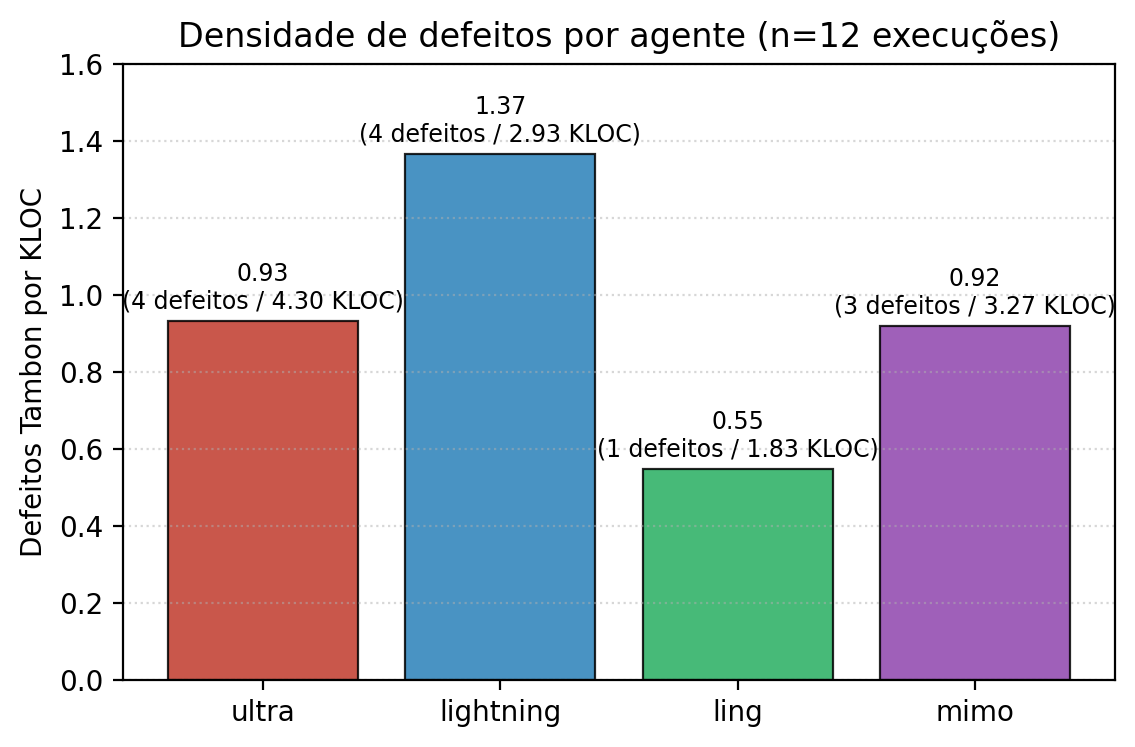
\includegraphics[width=0.62\textwidth]{fig1_densidade.png}
  \caption{Defect density per agent (defects/KLOC).}
  \label{fig:density}
\end{figure}

Descriptively, lightning presents the highest density (1.36/KLOC) and ling the lowest (0.55/KLOC) (Fig.~\ref{fig:density}). With $\leq$4 defects per agent, H1 is evaluated \textbf{descriptively} (wide Poisson CI); there is no power to claim significance.

\textbf{Category profile (RQ3/H2):}

\begin{table}[htbp]
  \centering
  \caption{Tambon category distribution per agent.}
  \label{tab:category}
  \begin{tabular}{lcccccc}
    \toprule
    Agent & incomplete\_gen & silly\_mistake & wrong\_input & non\_prompted & hallucinated & wrong\_attr \\
    \midrule
    ultra & 4 & 0 & 0 & 0 & 0 & 0 \\
    lightning & 0 & 1 & 0 & 1 & 1 & 1 \\
    ling & 0 & 0 & 1 & 0 & 0 & 0 \\
    mimo & 1 & 2 & 0 & 0 & 0 & 0 \\
    \bottomrule
  \end{tabular}
\end{table}

\begin{figure}[htbp]
  \centering
  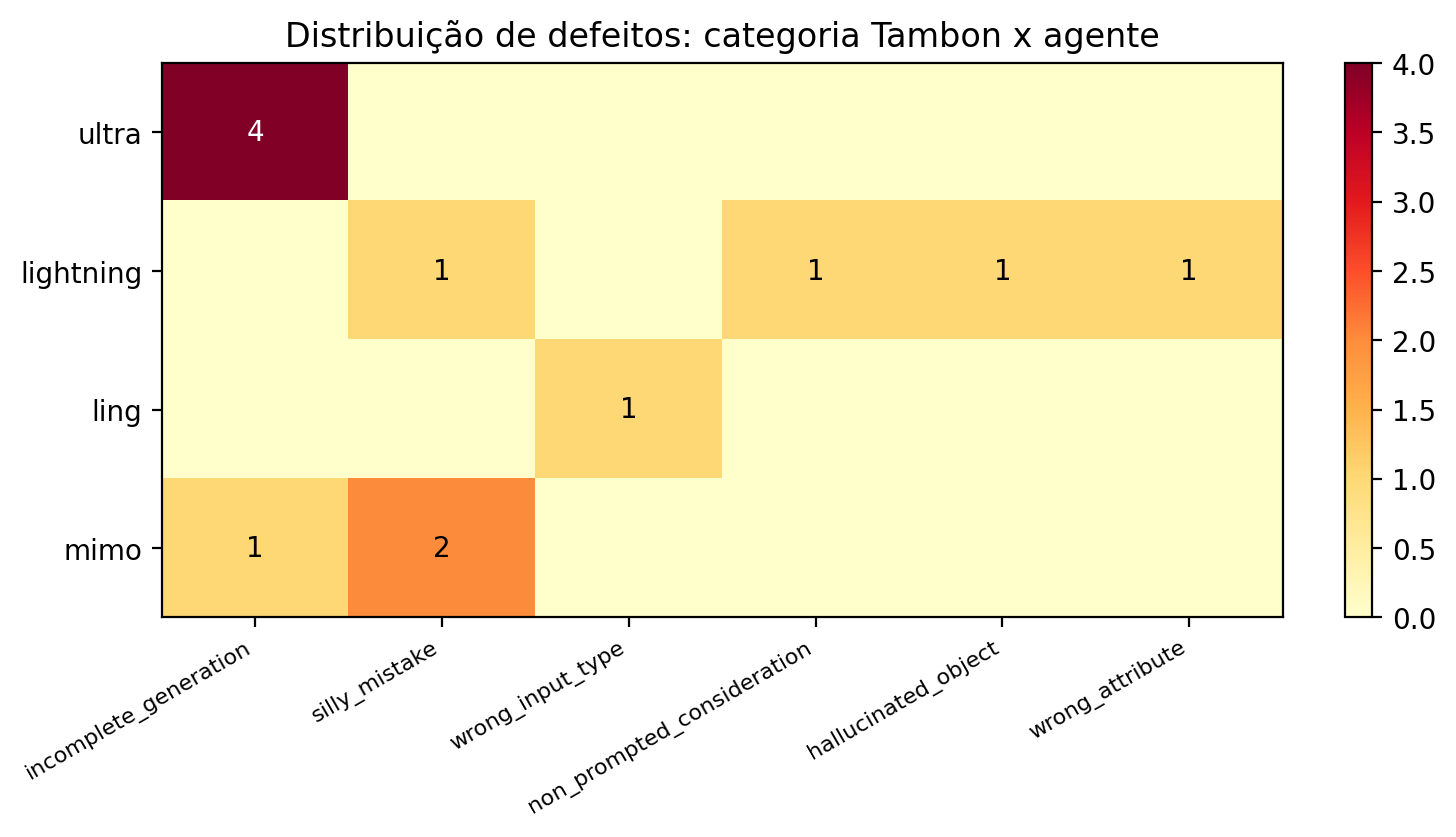
\includegraphics[width=0.62\textwidth]{fig2_heatmap_categoria_agente.png}
  \caption{Heatmap of agent $\times$ category defect distribution.}
  \label{fig:heatmap}
\end{figure}

The $\chi^2$ test of agent$\times$category independence resulted in \textbf{$\chi^2=25.7$, df=15, p=0.041, Cram\'er's $V$=0.85}---an \textbf{informative but not conclusive} association (expected cells $<$5; see Sec.~\ref{sec:method}). The \textbf{ultra} agent concentrated 100\% of defects in \texttt{incomplete\_generation} (pointwise Fisher exact \textbf{p=0.010} vs.\ others), the most sustainable finding; ling pointed toward \texttt{wrong\_input\_type} (p=0.083), mimo toward \texttt{silly\_mistake} (p=0.127), lightning with no dominant category. The heatmap (Fig.~\ref{fig:heatmap}) summarizes the distribution.

\subsection{Severity (RQ4)}

All 12 defects were \textbf{Blocker (8) or Critical (4)}; none Major/Minor (Fig.~\ref{fig:severity}). This concentration is expected and must be read with the \textbf{detection bias}: 10/12 deliveries did not boot, and a non-bootable deliverable has an automatically Blocker defect.

\begin{figure}[htbp]
  \centering
  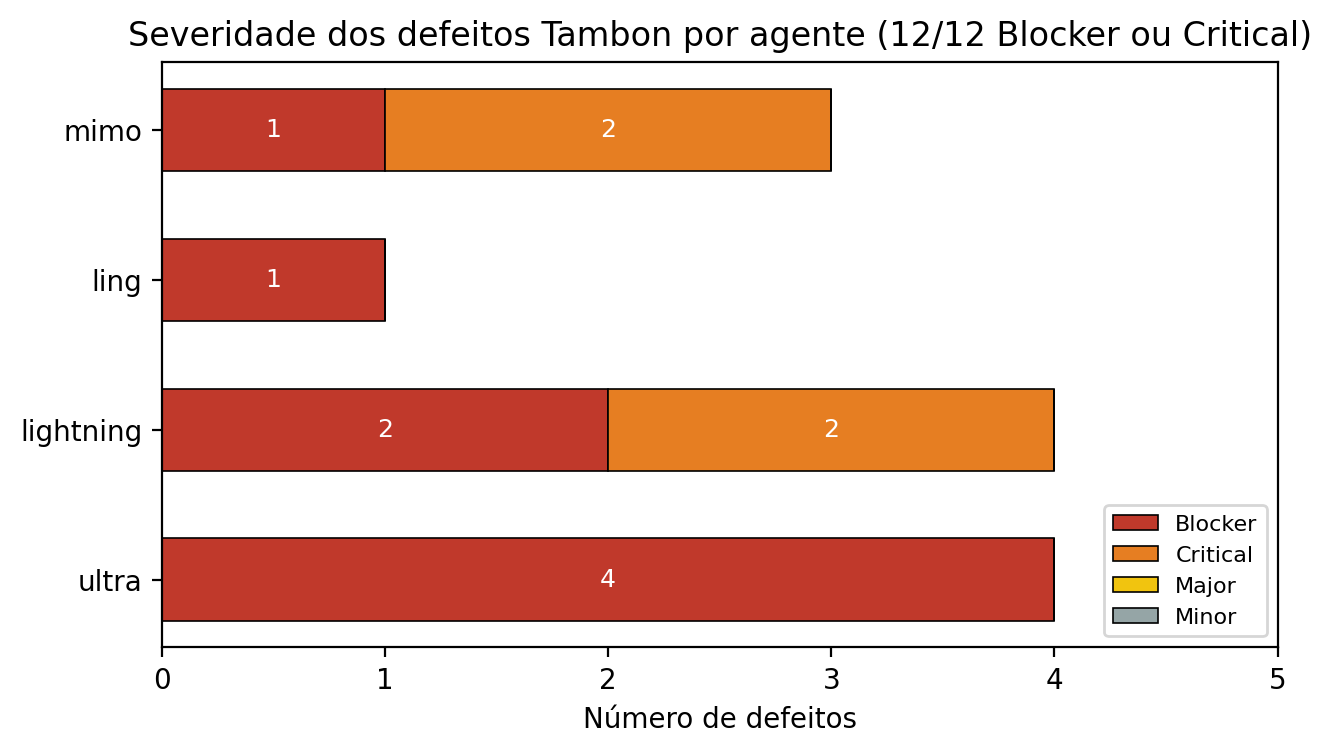
\includegraphics[width=0.62\textwidth]{fig5_severidade.png}
  \caption{Severity distribution of the 12 Tambon defects.}
  \label{fig:severity}
\end{figure}

\subsection{Recurring patterns}

\begin{table}[htbp]
  \centering
  \caption{Recurring defect patterns.}
  \label{tab:patterns}
  \begin{tabular}{lll}
    \toprule
    Pattern & Occurrences (in the 12) & Examples \\
    \midrule
    Missing dependency (\texttt{pydantic-settings}/\texttt{email-validator}) & 4 (+1 in pilot) & ultra e1/e3, mimo e1 \\
    \textit{passlib} 1.7.4 + \textit{bcrypt} $\geq$4.4 $\rightarrow$ 500 on \texttt{/auth/register} & 3 (+1 in pilot) & lightning e3, mimo e2/e3 \\
    Reproduction misconfiguration (alembic without \texttt{script\_location}) & 1 (+1 in pilot) & ultra e2 \\
    ``Ghost'' version (\texttt{pydantic==2.8.4} non-existent) & 1 & lightning e1 \\
    \bottomrule
  \end{tabular}
\end{table}

These patterns are \textbf{transferable across ``free'' models} of the same pipeline, suggesting a common ``quality trough'' at collection time.

\subsection{Testability---do the agent's tests detect the agent's defects? (RQ6/H3)}

$2\times2$ matrix (per defect; formal executions):

\begin{table}[htbp]
  \centering
  \caption{Defect detection: agent's own tests vs.\ oracle (per defect; $n=12$).}
  \label{tab:detect}
  \begin{tabular}{lccc}
    \toprule
    & Agent's tests: YES & Agent's tests: NO & Total \\
    \midrule
    \textbf{Oracle detected: YES} & 0 & \textbf{4} & 4 \\
    \textbf{Oracle detected: NO} \emph{(non-bootable)} & 0 & 8 & 8 \\
    \textbf{Total} & \textbf{0} & \textbf{12} & 12 \\
    \bottomrule
  \end{tabular}
\end{table}

\textbf{The tests generated by the agent itself detected none of the 12 Tambon defects (0/12; 0/18 matrix lines, including NFR and pilot)}. In the deliveries where the functionality was exercisable, the oracle detected \textbf{4/4} reachable defects (lightning/e3 $\times$2; mimo/e2, e3), while the agents' tests detected \textbf{0}---even when the agent's suite could run against the oracle. The 0-vs-4 pattern (the ``agent detected'' row entirely null) yields an extreme marginal Fisher statistic, reported as a \textbf{strong trend, not significance}, given the $n$ and the selection bias (3/12 bootable). The transversal, robust datum: \textbf{approval by the agent's own tests was, in no case, a guarantee of conformance with the oracle}---consistent with~\cite{C03,C04,C05,C06}.

\subsection{Inter-rater agreement and reproducibility (RQ7)}

Over 18 matrix items (independent, blinded double classification): \textbf{$\kappa$ category (Tambon) = 0.54 (moderate)}; \textbf{$\kappa$ severity = 0.91 (almost perfect)} (Fig.~\ref{fig:kappa}). The 6 category divergences concentrate on dependency-integration defects with multiple plausible classes (e.g., \texttt{silly\_mistake} $\times$ \texttt{wrong\_input\_type} in the \textit{passlib}+\textit{bcrypt} conflict), resolved in a recorded meeting. As to reproducibility (RQ7), 3/12 deliveries ran in a clean environment and with instructions; the rest failed due to dependencies, migration configuration, or non-existent versions (patterns of Sec.~\ref{sec:results}).

\begin{figure}[htbp]
  \centering
  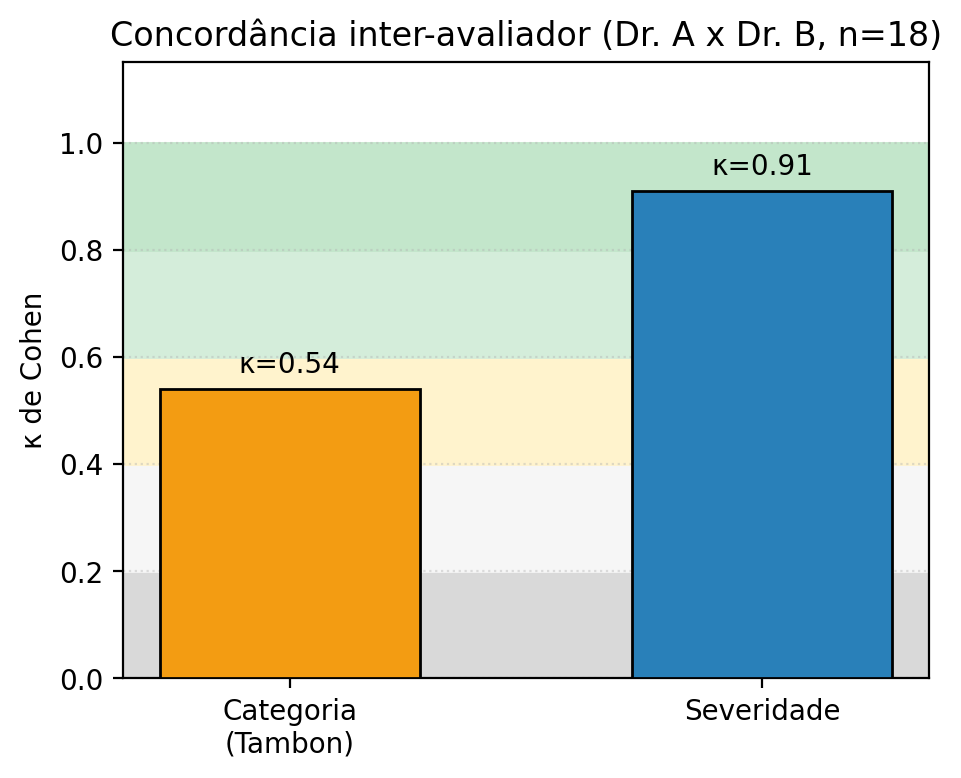
\includegraphics[width=0.62\textwidth]{fig4_kappa.png}
  \caption{Inter-rater agreement ($\kappa$) by matrix dimension.}
  \label{fig:kappa}
\end{figure}

\subsection{Variability across executions (RQ8)}

Where measurable (mimo), the \emph{pass rate} was \textbf{stable} across the two executions (0.15). Lightning had a single executable run (0.01). Ultra and ling produced no functional signal; variability is qualitative (all three ultra defects are \texttt{incomplete\_generation}).

\subsection{Global quality---functional $\neq$ non-functional (RQ5/H4)}

There is divergence across dimensions: deliveries that \textbf{boot} still fail 69--80 of the 81 tests (\emph{auth}/DB defects); deliveries that \textbf{do not boot} may pass the static NFRs (structural/reproducibility). A single index would collapse distinct dimensions---descriptively supporting H4.

\begin{figure}[htbp]
  \centering
  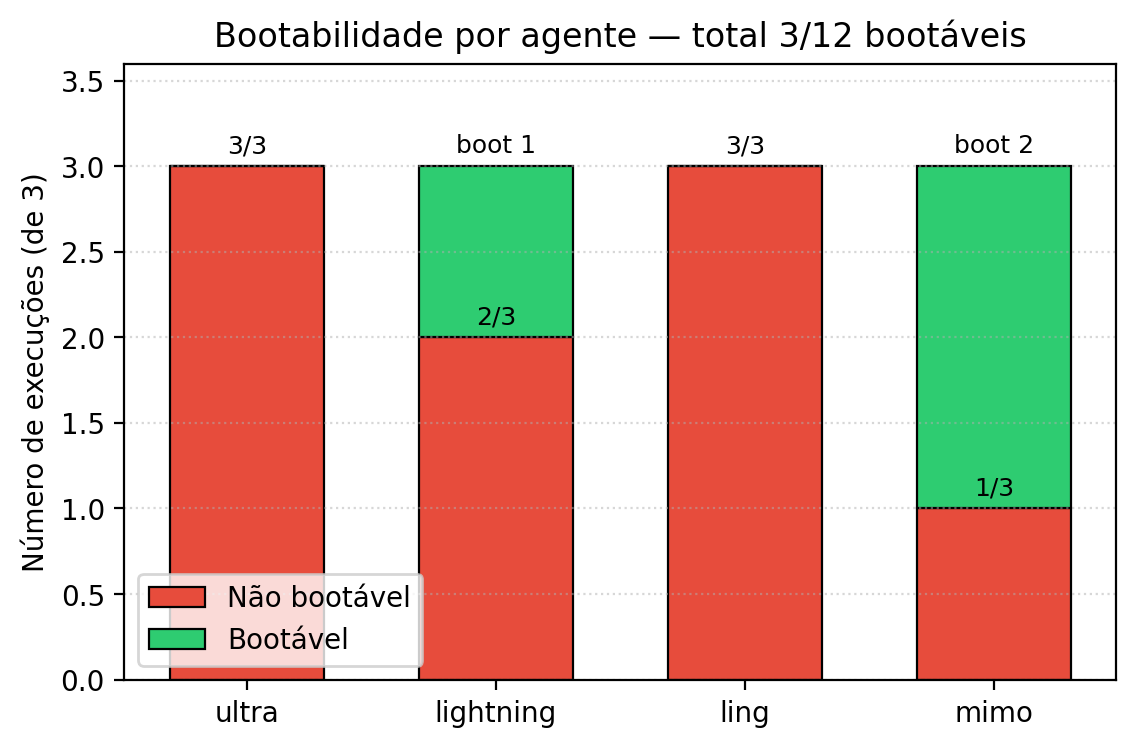
\includegraphics[width=0.62\textwidth]{fig3_bootabilidade.png}
  \caption{Bootability across the 12 deliveries.}
  \label{fig:boot}
\end{figure}

\section{Discussion}\label{sec:discussion}

\subsection{Interpretation of the main findings}

\textbf{Density and nature (RQ1--RQ4; H1, H2).} There are descriptive density differences (lightning 1.36; ultra 0.93; mimo 0.92; ling 0.55 defects/KLOC), with the most sustainable finding in the \textbf{ultra profile}: 100\% \texttt{incomplete\_generation} (p=0.010 Fisher). We interpret in terms of \textbf{profile}, not only quantity, consistent with evidence that AI and humans---and, here, different models---have distinct defect profiles~\cite{B03}. The $\chi^2$ points to an association (p=0.041, $V$=0.85) but \textbf{informative, not conclusive} (small $n$, cells $<$5). Thus, \textbf{H1 is neither rejected nor accepted} with this sample; \textbf{H2} finds pointwise support (ultra profile), without generalization.

\textbf{Severity (RQ4).} 100\% Blocker/Critical is expected and inflated by detection bias (10/12 non-bootable), preventing measurement of functional defects that would only appear in execution.

\textbf{Testability (RQ6/H3).} The most important result of the research: \textbf{0/12 defects detected by the agents' own tests}; \textbf{4/4 by the oracle} in the reachable ones. Self-approval $\neq$ independent validation---in line with the literature~\cite{C03,C04,C05,C06}. The methodological asymmetry (8/12 without functional oracle execution) limits the comparison and must be reported.

\textbf{Functional $\neq$ global (RQ5/H4).} Functional, structural, and security dimensions diverge; a single index would collapse them~\cite{D04}.

\textbf{Recurring patterns.} Missing dependencies, \textit{passlib}+\textit{bcrypt} conflict, migration misconfiguration, and ghost version concentrate the defects and repeat across distinct models---a common ``quality trough'' for free pipeline models at collection time, regardless of family. This extends, to the controlled scenario with free models, the findings of limited reproducibility/executability~\cite{F02} and unequal agent reliability~\cite{F05}.

\textbf{Variability (RQ8).} Limited where measurable; qualitative in general.

\subsection{Complementary laboratory study (non-evidential)}

\begin{quote}
\emph{Methodological caveat:} this subsection compares models and tasks \textbf{distinct} from the formal experiment (chat-LLMs, isolated function; not complete systems). Any convergence is only \textbf{indication}, never cross-evidence. It does not constitute evidence of the controlled experiment.
\end{quote}

In parallel, we conducted explorations with \textbf{chat-LLMs} (Oreate/Claude/Gemini---models different from the 4 treatments) on isolated QA tasks over a \texttt{create\_order} function with a 6-defect reference (EXP-001: detect; EXP-002: design tests). Findings: in \textbf{detection} (EXP-001), two models identified 6/6 and one 5/6 (missing the type/domain defect D1), echoing the \texttt{wrong input type} category~\cite{B01} and the omission of special cases~\cite{C06}; explicit boundaries ($>$ vs.\ $>=$) were detected by all. In \textbf{test generation} (EXP-002), coverage dropped to 5/6, 4/6, and 4/6; the most informative case was D1: a model that \emph{did not create a test} for the fractional quantity, although it had \emph{identified} the defect in EXP-001. This illustrates, in isolated scale, the same separation underlying RQ6/H3: \textbf{recognizing a defective condition and translating it into a test capable of revealing it are distinct abilities}---consistent with~\cite{C04} (29--60\% detection) and~\cite{C03}.

\subsection{Central limitations (honest reading)}\label{sec:limitations}

\begin{enumerate}
  \item \textbf{Restricted statistical power} ($n=12$; expected cells $<$5): H1--H3 are trends, not conclusions.
  \item \textbf{Small functionally evaluable fraction} (3/12 bootable): latent defects in non-bootable deliveries could not be measured.
  \item \textbf{Environment conditioning} (native validation, no Docker): deliveries configured only for container were treated as portability defects; we took care not to confuse ``defect'' with ``environment assumption''.
  \item \textbf{Manual classification:} moderate category $\kappa$ (0.54); resolutions recorded, but the taxonomy over integration defects remains ambiguous.
  \item \textbf{``Free'' models and collection time:} results describe these specific models at collection date; route/version changes alter the picture.
  \item \textbf{Small defect sample and Blocker bias} (due to non-bootability).
  \item \textbf{No generalization:} a single target system (tasks) and stack (Python/FastAPI/PostgreSQL).
\end{enumerate}

\subsection{Synthesis}

In the controlled scenario, agents of ``free'' models in agent mode produced complete systems with low execution rate (3/12), defects concentrated in few recurring patterns, and no full conformance with the oracle. The most sustainable evidence is the \textbf{ultra's incomplete-generation profile}; the most general is the \textbf{common quality trough} among free models of the same pipeline. The exploratory, non-evidential laboratory reinforces the separation between \emph{detecting} and \emph{testing}. The results \emph{do not} support either ``AI does not work'' or ``AI replaces QA'': they support that, \textbf{under controlled requirements and with an independent oracle, the quality delivered by these agents at collection time fell below the functional minimum in 9 of 12 executions}, and that approval by the agents' own tests is no substitute for independent validation.

\section{Conclusion and Future Work}\label{sec:conclusion}

\textbf{Conclusion.} This study contributes a controlled, prospective, and reproducible experiment that combines---for the first time, as far as the review reaches---complete-system generation by different AI agents from the same requirement, multiple executions, an independent oracle, and simultaneous evaluation of functionality, defects, security, maintainability, reproducibility, and testability. Among the results, we highlight: low executability (3/12); a defect profile concentrated in recurring patterns transferable across free models (``quality trough''); and the \textbf{non-detection of defects by the agent's own tests} (0/12) versus oracle detection (4/4 reachable), reinforcing that self-approval $\neq$ independent validation. With due rigor of neutrality, the data---not a premise---support these readings, within the statistical-power and generalization limitations declared in Sec.~\ref{sec:limitations}.

\textbf{Future work.} (i)~\textbf{Sample expansion} (more executions and/or Docker execution on the production machine) to raise expected cells $\geq$5 and give power to the $\chi^2$; (ii)~\textbf{running the deliverables' containers} on the production machine (validating the mandatory Docker layer); (iii)~\textbf{extension to more models/families and to distinct complete agents} (also comparing the agent tool, not only the model); (iv)~formalize a full \textbf{pre-registration} (already started in a private repository) for the expanded design; (v)~\textbf{longitudinal study} verifying whether the ``quality trough'' persists with model updates; (vi)~\textbf{evaluation of authorship/quality of minimal human intervention}, contrasting with autonomous generation; (vii)~\textbf{pre-registered laboratories} (EXP-003 and EXP-bridge) to test the type/domain-validity-range and boundary hypothesis, without contamination with the formal experiment; and (viii)~a full formal \textbf{SLR} (the current one is intentionally lean and documented as a research artifact).

\section*{Data and Code Availability}

The preprint record at Zenodo (DOI: \href{https://zenodo.org/records/22551156}{10.5281/zenodo.22551156}, CC-BY-4.0) hosts the manuscript version of this study. The figure-generation script and the aggregated data used in Figures~\ref{fig:density}--\ref{fig:severity} are available in the publicly accessible research repository linked to that record. The executable specification and the independent oracle suite are intentionally kept private for neutrality and security reasons; after peer-reviewed acceptance, curated artifacts will be deposited with a DOI under CC-BY-4.0, and raw execution logs (containing environment/app credentials) remain restricted with documented justification.

\begin{thebibliography}{99}\label{sec:refs}

\bibitem{A01} HOU, X. et al. \emph{Large Language Models for Software Engineering: A Systematic Literature Review}. ACM Transactions on Software Engineering and Methodology, v.~33, n.~8, art.~220, 2024. DOI: \texttt{10.1145/3695988}.

\bibitem{A02} UMAMA et al. \emph{LLM-Based Code Generation: A Systematic Literature Review With Technical and Demographic Insights}. IEEE Access, v.~13, pp.~194915--194939, 2025. DOI: \texttt{10.1109/ACCESS.2025.3631952}.

\bibitem{B01} TAMBON, F. et al. \emph{Bugs in Large Language Models Generated Code: An Empirical Study}. Empirical Software Engineering, v.~30, art.~65, 2025. DOI: \texttt{10.1007/s10664-025-10614-4}.

\bibitem{B02} DOU, S. et al. \emph{What's Wrong with Your Code Generated by Large Language Models? An Extensive Study}. arXiv:2407.06153 {[cs.SE]}, 2024.

\bibitem{B03} COTRONEO, D.; IMPROTA, C.; LIGUORI, P. \emph{Human-Written vs.\ AI-Generated Code: A Large-Scale Study of Defects, Vulnerabilities, and Complexity}. IEEE ISSRE 2025, pp.~252--263. DOI: \texttt{10.1109/ISSRE66568.2025.00035}.

\bibitem{B04} OUYANG, S.; ZHANG, J. M.; HARMAN, M.; WANG, M. \emph{An Empirical Study of the Non-Determinism of ChatGPT in Code Generation}. ACM Transactions on Software Engineering and Methodology, v.~34, n.~2, art.~42, 2025. DOI: \texttt{10.1145/3697010}.

\bibitem{C01} WANG, J. et al. \emph{Software Testing With Large Language Models: Survey, Landscape, and Vision}. IEEE Transactions on Software Engineering, v.~50, n.~4, pp.~911--936, 2024. DOI: \texttt{10.1109/TSE.2024.3368208}.

\bibitem{C02} BEER, A. et al. \emph{Examination of Code generated by Large Language Models}. arXiv:2408.16601 {[cs.SE]}, 2024.

\bibitem{C03} ALVES, V. A.; SANTOS, C.; BEZERRA, C. I. M.; MACHADO, I. \emph{Detecting Test Smells in Python Test Code Generated by LLM: An Empirical Study with GitHub Copilot}. SBES 2024, CBSoft. DOI: \texttt{10.5753/sbes.2024.3561}.

\bibitem{C04} YANG, L. et al. \emph{On the Evaluation of Large Language Models in Unit Test Generation}. ASE 2024. DOI: \texttt{10.1145/3691620.3695529}.

\bibitem{C05} ZHAO, J.; ZHOU, S.; COHEN, E. \emph{Do Coverage and Mutation Scores of LLM-Generated Test Suites Correlate with Their Effectiveness? (Replicability Study)}. ISSTA 2026. DOI: \texttt{10.1145/3832093}.

\bibitem{C06} WALCZAK, J.; TOMALAK, P.; LASKOWSKI, A. \emph{Impact of code context and prompting strategies on automated unit test generation with modern general-purpose large language models}. Journal of Systems and Software, v.~237, art.~112834, 2026. DOI: \texttt{10.1016/j.jss.2026.112834}.

\bibitem{D01} TOSI, D. \emph{Studying the Quality of Source Code Generated by Different AI Generative Engines: An Empirical Evaluation}. Future Internet, v.~16, n.~6, art.~188, 2024. DOI: \texttt{10.3390/fi16060188}.

\bibitem{D02} MOLISON, A. S. et al. \emph{Is LLM-Generated Code More Maintainable \& Reliable than Human-Written Code?}. arXiv:2508.00700 {[cs.SE]}, 2025.

\bibitem{D03} BAUER, J.; LINDEMAN, L.; REILLY, L.; RODRIGUEZ, M. \emph{Does GitHub Copilot improve code quality? Here's what the data says}. GitHub Customer Research, 2024. Available at: \url{https://github.blog/news-insights/research/does-github-copilot-improve-code-quality-heres-what-the-data-says/}.

\bibitem{D04} SUN, X.; ST{\AA}HL, D.; SANDAHL, K.; KESSLER, C. \emph{Quality assurance of LLM-generated code: Addressing non-functional quality characteristics}. Journal of Systems and Software, v.~238, art.~112885, 2026. DOI: \texttt{10.1016/j.jss.2026.112885}.

\bibitem{D05} LIU, Y. et al. \emph{Debt Behind the AI Boom: A Large-Scale Empirical Study of AI-Generated Code in the Wild}. arXiv:2603.28592 {[cs.SE]}, 2026.

\bibitem{E01} FU, Y. et al. \emph{Security Weaknesses of Copilot-Generated Code in GitHub Projects: An Empirical Study}. ACM Transactions on Software Engineering and Methodology, v.~34, n.~8, 2025. DOI: \texttt{10.1145/3716848}.

\bibitem{E02} MORKONDA, S. G.; SELIM, M.; ASSAL, H. \emph{Security of LLM-generated Code: A Comparative Analysis}. arXiv:2605.23091 {[cs.CR]}, 2026.

\bibitem{E03} KHARMA, M. et al. \emph{An Empirical Evaluation of LLM-Generated Code Security Across Prompting Methods}. arXiv:2605.24298 {[cs.CR]}, 2026.

\bibitem{F01} HORIKAWA, K. et al. \emph{Agentic Refactoring: An Empirical Study of AI Coding Agents}. arXiv:2511.04824 {[cs.SE]}, 2025.

\bibitem{F02} VANGALA, B. P.; ADIBIFAR, A.; GEHANI, A.; MALIK, T. \emph{AI-Generated Code Is Not Reproducible (Yet): An Empirical Study of Dependency Gaps in LLM-Based Coding Agents}. arXiv:2512.22387 {[cs.SE]}, 2025/2026. DOI: \texttt{10.48550/arXiv.2512.22387}.

\bibitem{F03} BELOZEROV, V.; BARCLAY, P. J.; SAMI, A. \emph{Secure coding with AI---from detection to repair}. Empirical Software Engineering, v.~31, art.~93, 2026. DOI: \texttt{10.1007/s10664-026-10812-8}.

\bibitem{F04} EHSANI, R. et al. \emph{Where Do AI Coding Agents Fail? An Empirical Study of Failed Agentic Pull Requests in GitHub}. MSR 2026, pp.~807--811. DOI: \texttt{10.1145/3793302.3793579}.

\bibitem{F05} OUKHAY, I.; BEGOUG, M.; CHOUCHEN, M.; OUNI, A. \emph{When AI Code Doesn't Stick: An Empirical Study on Reverted Changes Introduced by AI Coding Agents}. MSR 2026, pp.~847--851. DOI: \texttt{10.1145/3793302.3793587}.

\end{thebibliography}

\end{document}